The merge sort is a divided and conquer comparison sort, having both a serial and parallel version. The idea behind the merge sort, is to first divide the input data into 1 element subsets. Then each pair of subsets are merged by sort, creating a new smaller set of sorted subsets. The merging step is carried out until the number of subsets reach 1, representing the final sorted output data. A visual representation of the merge sort is seen in \cref{fig:sort_merge}.

\begin{figure}[ht]
	\centering
	\fbox{
		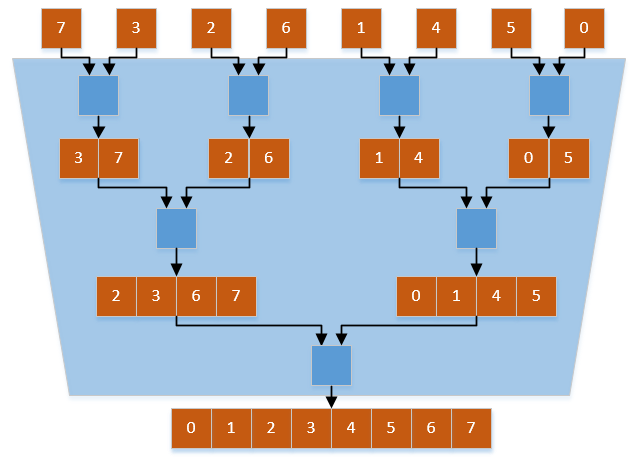
\includegraphics[width=0.5\textwidth]{figs/algorithm/sort_merge.png}}
	\caption{Merge sort}
	\label{fig:sort_merge}
\end{figure}  

The implementation of serial merge sort, is rather simple and can be done using recursion. That approach cannot be used for a parallel implementation, as load unbalance happens when few thread have to merge large arrays. Another approach is therefore necessary for a parallel merge sort. The parallel strategy consist of 3 stages; merge-per-thread, merge-per-block and merge-by-blocks. The first stage is carried out when there are a lot of small merges required. Each merge is allocated to one thread, thereby there are a lot of individual threads working in parallel utilizing the GPU. When the merges reach a size and number where only few threads will work a lot, the merge-per-block stage is enabled. In this stage each merge is carried out by multiple threads in a block. Each thread in a block is allocated one array element from one of the two merging arrays. Each thread then calculates the position of its element in the merged array, and writes the element to that position. This procedure is visual represented in \cref{fig:sort_merge_per_block}.     

\begin{figure}[ht]
	\centering
	\fbox{
		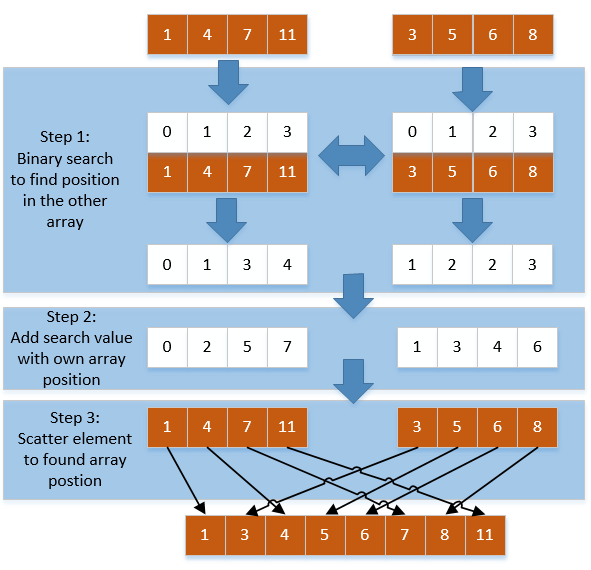
\includegraphics[width=0.5\textwidth]{figs/algorithm/sort_merge_per_block.png}}
	\caption{Merge sort merge-per-block}
	\label{fig:sort_merge_per_block}
\end{figure}  

First each thread uses binary search to find its elements position in the other merge array. Second that position is added with the elements own array position resulting in the array position in the final merged array. Third and last the thread writes the element to the merged array, to the found position. The last stage of the merge sort is the merge-by-blocks, is stage is carried out when the merge arrays is to large for a single block, so when each element can not be assigned its own thread. The merging arrays are divided across thread blocks, thereby having multiple blocks working on the same merge. The merge sort, in its serial implementation, have a work and step complexity of $\mathcal{O}(n~log~n)$. In the parallel implementation, there is a work complexity of $\mathcal{O}(n~log~n)$ and a step complexity of $\mathcal{O}(log^2~n)$, thereby working better than both the serial implementation and the odd-even sort.  